\chapter{Arhitektura i dizajn sustava}
		

	\textnormal{Pri procesu izbora arhitekture naše web aplikacije fokusirali smo se na klijent-server strukturu uz mogućnost odvojenih podsustava. U takvoj strukturi web poslužitelj osnova je rada web aplikacije. Njegova primarna zadaća je komunikacija klijenta s aplikacijom putem HTTP (\textit{engl. Hyper Text Transfer Protocol}) protokola. Korisnik šalje zahtjeve poslužitelju putem web preglednika. Web preglednik je program koji korisniku omogućuje pregled web-stranica i multimedijalnih sadržaja vezanih uz njih tako što stranicu pisanu u kodu interpretira na način da je razumljiva korisniku. Na temelju poslanih zahtjeva web aplikacija pristupa bazi podataka te vraća odgovor putem poslužitelja u obliku HTML dokumenta koji je vidljiv u pregledniku.}

	\begin{figure}[H]
		\centering
		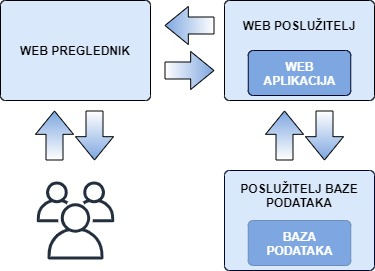
\includegraphics[scale=0.7]{slike/Arhitektura} \\
		\caption{ Organizacija sustava}
		\label{fig:arhitektura}
	\end{figure}

	\textnormal{Na temelju navedenih glavnih značajki i nadalje razrađenih obilježja odlučili smo se arhitekturu sustava bazirati na arhitekturnom stilu model-pogled-upravitelj (\textit{engl. Model-View-Controller, MVC}). Kod MVC stila, korisničko sučelje je odvojeno od ostatka sustava što nam omogućuje raspodjelu u odvojene timove tijekom rada na projektu. Mnogi programski okviri su izrađeni s MVC arhitekturom na umu, što omogućuje brži i jednostavniji razvoj aplikacije. Razinska kohezija elemenata postiže se kroz tri sloja, jednog na strani klijenta koji se naziva pogled (\textit{engl. view}) i dva na poslužiteljskoj strani, koji se nazivaju upravitelj (\textit{engl. controller}) i model (\textit{engl. model}), što nam uz povećanu koheziju i smanjivanje međuovisnosti omogućuje i fleksibilnost. Također smo izabrali ovaj arhitekturni stil zbog njegove mogućnosti jednostavne ponovne uporabe i nadogradnje pojedinačnih dijelova sustava, pošto se dodavanjem novih modela ili pogleda može brzo i jednostavno promijeniti aplikaciju. Time se pozitivno utječe i na planiranje zastare aplikacije, uz korištenje dobro poznatih tehnologija i jezika koji će biti detaljnije razrađeni u nastavku. Podjelom na navedene podsustave pojednostavili smo i testiranje tijekom izrade aplikacije jer se razni dijelovi sustava mogu neovisno testirati. Izborom web aplikacije pobrinuli smo se i za prenosivost, pošto se aplikaciji može pristupiti s velikog broja uređaja putem različitih web preglednika.}\\
	
	\textnormal{Negativna karakteristika MVC arhitekture može biti njezina glomaznost u pogledu velike količine datoteka što može usporiti sustav, no to ne smatramo problemom za ovaj projekt pošto je manjeg opsega.}\\
	
	\begin{figure}[H]
		\centering
		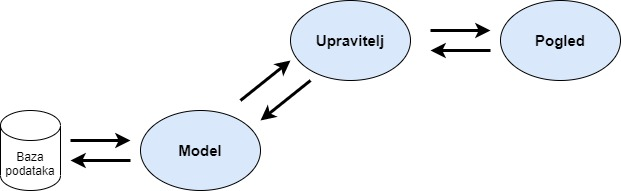
\includegraphics[scale=0.5]{slike/MVC} \\
		\caption{ MVC Arhitektura}
		\label{fig:arhitekturaMCV}
	\end{figure}

	\textnormal{U skladu s odabranom arhitekturom, aplikacija će biti razvijena u tri velike nezavisne komponente: pogled kroz \textit{front-end} sustav, te upravitelj i model kroz \textit{back-end} sustav i bazu podataka.}\\
	
	\textnormal{\textit{Front-end} predstavlja korisničko sučelje s kojim korisnik ima direktnu interakciju. Implementiran je pomoću programskog okvira Angular koristeći TypeScript, JavaScript, HTML i CSS. Za Angular smo se odlučili jer omogućava dizajniranje fleksibilnih komponenti visoke razine ponovne upotrebljivosti uz veliku responzivnost i interaktivnost. Uloge Angular servisa u ovoj aplikaciji su dostaviti sve potrebne podatke i skripte web poslužitelju korisnika, komunikacija s back end servisom i izvođenje vlastitih procesa koji su nužni za pravilan rad korisničkog sučelja. Razdvajanjem \textit{front-end} i \textit{back-end} servisa omogućavamo fokus na razvoj odličnog korisničkog sučelja što je bitan faktor korisnicima pri odabiru naše igre kao jedne od mnogo dostupnih.}\\
	
	\textnormal{\textit{Back-end} predstavlja servis koji upravlja \textit{front-end} servisom i dostavlja podatke korisniku te je zato centralna točka GeoFighter aplikacije. Implementiran je pomoću programskog okvira SpringBoot koristeći programski jezik Java. Omogućava pristup bazi podataka, komunikaciju HTTP zahtjevima te sadržava logiku i funkcionalnosti GeoFighter igre. Struktura \textit{back-end} servisa se fokusira na smanjivanje međuovisnosti sadržaja i izbjegava opću međuovisnost. Razdvajanjem \textit{front-end} i \textit{back-end} servisa smanjujemo opterećenost \textit{back-end} servisa}\\
	
	\textnormal{Baza podataka je trajno spremište svih podataka koje GeoFighter aplikacija treba sadržavati. Ona komunicira isključivo s \textit{back-end} servisom. Baza podataka je relacijskog tipa te je implementirana koristeći Postgres. Postgres baza podataka je odličan izbor za baze podataka male do srednje veličine te je vrlo fleksibilan izbor za zahtjeve koje ova aplikacija izvršava.}\\
	
	\begin{figure}[H]
		\centering
		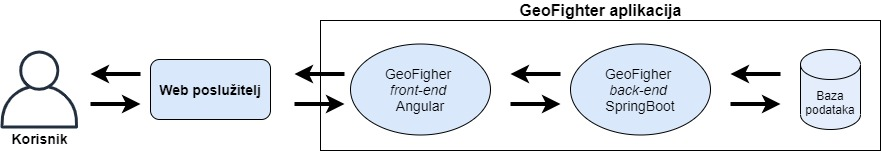
\includegraphics[scale=0.5]{slike/strukturaGF} \\
		\caption{Skica arhitekture sustava}
		\label{fig:arhitekturaGF}
	\end{figure}
	
	
				
		\section{Baza podataka}
			
			
		\textnormal{Za potrebe našeg sustava koristiti ćemo relacijsku bazu podataka koja svojom strukturom 	olakšava modeliranje stvarnog svijeta. Gradivna jedinka baze je relacija, odnosno tablica koja je definirana svojim imenom i skupom atributa, dok su odnosi između relacija definirani vezama. Zadaća baze podataka je brza i jednostavna pohrana, izmjena i dohvat podataka za daljnju obradu.\\Baza podataka ove aplikacije sastoji se od slijedećih tablica:}
		
		\begin{packed_item}
			\item \textnormal{Users}
			\item \textnormal{Tokens}
			\item \textnormal{Refresh\textunderscore token}
			\item \textnormal{Roles}
			\item \textnormal{Privileges}
			\item \textnormal{Roles\textunderscore privileges}
			\item \textnormal{Location\textunderscore cards}
			\item \textnormal{User\textunderscore card}
			\item \textnormal{Fights}
			\item \textnormal{User\textunderscore  card\textunderscore fight}
		\end{packed_item}
		
			\subsection{Opis tablica}
			

				\textnormal{\textbf{Users} \quad Ovaj entitet sadržava sve važne informacije o korisniku aplikacije koje bilježi atributima navedenim u tablici. U vezi je \textit{One-to-Many} s entitetima Tokens, Fights, Location\textunderscore cards i User\textunderscore card preko atributa user\textunderscore id. Također je u vezi \textit{Many-to-One} s entitetom Roles preko atributa role\textunderscore id.} \\
				
				\begin{longtabu} to \textwidth {|X[6, 3]|X[6, l]|X[20, l]|}
					
					\hline \multicolumn{3}{|c|}{\textbf{users}}	 \\[3pt] \hline
					\endfirsthead
					
					\hline \multicolumn{3}{|c|}{\textbf{users}}	 \\[3pt] \hline
					\endhead
					
					\hline 
					\endlastfoot
					
					\textbf{user\textunderscore id} & BIGSERIAL	&  	jedinstveni identifikator korisnika	\\ \hline
					email & VARCHAR & email adresa korisnika \\ \hline
					username & VARCHAR & korisničko ime \\ \hline
					password & VARCHAR & lozinka korisnika \\ \hline
					photourl & VARCHAR & poveznica na fotografiju profila \\ \hline
					created\textunderscore time & TIMESTAMP & trenutak stvaranja korisničkog računa  \\ \hline 
					current\textunderscore location & BYTEA	&  	trenutna lokacija korisnika	\\ \hline 
					elo\textunderscore score & INT4 & rang korisnika prema elo sustavu \\ \hline
					enabled & BOOLEAN & zastavica potvrde email adrese\\ \hline
					losses & INT4 & broj izgubljenih igara \\ \hline
					wins & INT4 & broj pobijeđenih igara \\ \hline
					online & BOOLEAN & zastavica prisutnosti korisnika \\ \hline
					forced\textunderscore timeout\textunderscore end & TIMESTAMP & trenutak mogućeg povratka u igru u slučaju privremenog isključenja \\ \hline
					cartographer\textunderscore status	& INT4 &   oznaka statusa pri prijavi za kartografa 	\\ \hline 
					iban & VARCHAR & IBAN bankovnog računa kartografa \\ \hline			
					id\textunderscore card\textunderscore photourl & VARCHAR & poveznica na fotografiju osobne iskaznice \\ \hline
					\textit{role\textunderscore id} & INT8 &  jedinstveni identifikator uloge (roles.role\textunderscore id)	\\ \hline 
					
					
				\end{longtabu}
			
				
				\textnormal{\textbf{Tokens} \quad Ovaj entitet sadržava sve važne informacije o tokenima koji se koriste za autentifikaciju korisnika. Atributi koje posjeduje su jedinstveni identifikator tokena, njegova vrijednost, datum isticanja te oznaku korisnika kojem pripada. U vezi je \textit{Many-to-One} s entitetom Users preko atributa "user\textunderscore user\textunderscore id".} \\
			
			
			
				\begin{longtabu} to \textwidth {|X[6, l]|X[6, l]|X[20, l]|}
					
					\hline \multicolumn{3}{|c|}{\textbf{tokens}}	 \\[3pt] \hline
					\endfirsthead
					
					\hline \multicolumn{3}{|c|}{\textbf{tokens}}	 \\[3pt] \hline
					\endhead
					
					\hline 
					\endlastfoot
					
					\textbf{id} & BIGSERIAL	&  	jedinstveni identifikator tokena 	\\ \hline
					expiry\textunderscore date	& TIMESTAMP &   datum isticanja tokena	\\ \hline 
					token & VARCHAR &  vrijednost tokena \\ \hline  
					\textit{"user\textunderscore user\textunderscore id"} & INT8 &  jedinstvena oznaka korisnika (users.user\textunderscore id) 	\\ \hline 
					
					
				\end{longtabu}
			
				\textnormal{}
			
				\textnormal{\textbf{Refresh\textunderscore token} \quad Ovaj entitet sadržava sve važne informacije o obnavljanju tokena koji služe za autentifikaciju korisnika. Atributi koje posjeduje su jedinstveni identifikator tokena, njegova nova vrijednost te datum stvaranja.} \\
				
			\begin{longtabu} to \textwidth {|X[6, l]|X[6, l]|X[20, l]|}
				
				\hline \multicolumn{3}{|c|}{\textbf{refresh\textunderscore token}}	 \\[3pt] \hline
				\endfirsthead
				
				\hline \multicolumn{3}{|c|}{\textbf{refresh\textunderscore token}}	 \\[3pt] \hline
				\endhead
				
				\hline 
				\endlastfoot
				
				\textbf{id} & BIGSERIAL &  	jedinstveni identifikator tokena (tokens.id) 	\\ \hline
				created\textunderscore date	& TIMESTAMP &   datum stvaranja tokena	\\ \hline 
				token & VARCHAR & vrijednost tokena  \\ \hline 
				
				
				
			\end{longtabu}
		
			\textnormal{}
		
			\textnormal{\textbf{Roles} \quad Ovaj entitet sadržava sve važne informacije vezane uz ulogu koju određeni korisnik može imati, a one su administrator, kartograf ili igrač. Atributi koje posjeduje su jedinstveni identifikator uloge i njezin naziv. U vezi je \textit{One-to-Many} s entitetom Users preko atributa role\textunderscore id. Također je u vezi \textit{Many-to-Many} s entitetom Privileges preko spojne tablice roles\textunderscore privileges.} \\
		
			\begin{longtabu} to \textwidth {|X[6, l]|X[6, l]|X[20, l]|}
				
				\hline \multicolumn{3}{|c|}{\textbf{roles}}	 \\[3pt] \hline
				\endfirsthead
				
				\hline \multicolumn{3}{|c|}{\textbf{roles}}	 \\[3pt] \hline
				\endhead
				
				\hline 
				\endlastfoot
				
				\textbf{role\textunderscore id} & INT8	&  	jedinstveni identifikator uloge 	\\ \hline
				name	& VARCHAR &   naziv uloge	\\ \hline 
							
				
			\end{longtabu}
		
			\eject
		
			\textnormal{\textbf{Privileges} \quad Ovaj entitet sadržava sve važne informacije o povlasticama koje uloge mogu imati. Atributi koje posjeduje su jedinstveni identifikator povlastice i njen naziv. U vezi je \textit{Many-to-Many} s entitetom Roles preko spojne tablice roles\textunderscore privileges.} \\
		
			\begin{longtabu} to \textwidth {|X[6, l]|X[6, l]|X[20, l]|}
				
				\hline \multicolumn{3}{|c|}{\textbf{privileges}}	 \\[3pt] \hline
				\endfirsthead
				
				\hline \multicolumn{3}{|c|}{\textbf{privileges}}	 \\[3pt] \hline
				\endhead
				
				\hline 
				\endlastfoot
				
				\textbf{privilege\textunderscore id} & INT8	&  	jedinstveni identifikator povlastice 	\\ \hline
				name	& VARCHAR &   naziv povlastice	\\ \hline 
								
				
			\end{longtabu}
		
			\textnormal{}
		
			\textnormal{\textbf{Roles\textunderscore privileges} \quad Ova tablica nastaje zbog \textit{Many-to-Many} veze između entiteta Roles i Privileges. Sadrži njihove primarne ključeve te je time povezana s njima. Prikazuje koje uloge imaju koje povlastice.} \\
			
			\begin{longtabu} to \textwidth {|X[6, l]|X[6, l]|X[20, l]|}
				
				\hline \multicolumn{3}{|c|}{\textbf{roles\textunderscore privileges}}	 \\[3pt] \hline
				\endfirsthead
				
				\hline \multicolumn{3}{|c|}{\textbf{roles\textunderscore privileges}}	 \\[3pt] \hline
				\endhead
				
				\hline 
				\endlastfoot
				
				\textbf{\textit{role\textunderscore id}} & INT8 & jedinstveni identifikator uloge (roles.role\textunderscore id) \\ \hline
				\textbf{\textit{privilege\textunderscore id}} & INT8	&  	jedinstveni identifikator povlastice (privileges.privilege\textunderscore id) 	\\ \hline
				
						
				
			\end{longtabu}
		
			\textnormal{}
		
			\textnormal{\textbf{Location\textunderscore cards} \quad Ovaj entitet sadržava sve važne informacije o karticama lokacije. Atributi koje posjeduje su navedeni u tablici. Važno je istaknuti atribute uncommonness, difficulty i population. Oni će određivati jačinu kartice tijekom borbe. Njihovim izborom postignuta je ravnoteža pri dodjeljivanju jačine kartice jer će lokacije koje su teže dostupne obično imati manju naseljenost. U vezi je \textit{Many-to-Many-to-Many} s entitetima Fights i Users preko spojne tablice User\textunderscore card\textunderscore fight. Također je u vezi \textit{Many-to-One} s entitetom Users preko atributa accepted\textunderscore by\textunderscore user \textunderscore id i atributa created\textunderscore by\textunderscore user \textunderscore id.} \\
		
			\begin{longtabu} to \textwidth {|X[6, 4]|X[6, l]|X[20, l]|}
				
				\hline \multicolumn{3}{|c|}{\textbf{location\textunderscore cards}}	 \\[3pt] \hline
				\endfirsthead
				
				\hline \multicolumn{3}{|c|}{\textbf{location\textunderscore cards}}	 \\[3pt] \hline
				\endhead
				
				\hline 
				\endlastfoot
				
				\textbf{lcd\textunderscore id} & INT8	&  	jedinstveni identifikator kartice lokacije 	\\ \hline
				name	& VARCHAR &   naziv lokacije	\\ \hline 
				accepted & BOOLEAN & zastavica koja označava je li lokacija odobrena \\ \hline
				created\textunderscore at & TIMESTAMP & trenutak stvaranja kartice lokacije \\ \hline
				description & TEXT & opis lokacije \\ \hline
				enabled\textunderscore date & TIMESTAMP & trenutak odobravanja kartice lokacije \\ \hline
				location & BYTEA & stvarna lokacija koju označava kartica lokacije \\ \hline
				check\textunderscore needed & BOOLEAN & zastavica koja označava potrebu za dodatnom potvrdom kartice lokacije \\ \hline
				photo & VARCHAR & digitalni zapis fotografije lokacije \\ \hline
				uncommonness & INT & atribut koji označava rijetkost kartice \\ \hline
				difficulty & INT & atribut koji označava težinu dostupnosti lokacije \\ \hline
				population & INT & atribut koji označava naseljenost lokacije \\ \hline
				\textit{accepted\textunderscore by\textunderscore user \textunderscore id} & INT8 & jedinstveni identifikator kartografa koji je odobrio karticu lokacije (users.user\textunderscore id) \\ \hline
				\textit{created\textunderscore by\textunderscore user \textunderscore id} & INT8 & jedinstveni identifikator igrača koji je prijavio karticu lokacije (users.user\textunderscore id) \\ \hline				
				
				
			\end{longtabu}
		
			\textnormal{}
		
			\textnormal{\textbf{User\textunderscore card} \quad Ovaj entitet sadržava sve informacije o kartici koju posjeduje neki igrač. Atributi koje posjeduje su jedinstveni identifikator korisnika i kartice koju posjeduje, trenutak kada se kartica može ponovo koristit u borbi te koeficijent koji utječe na smanjenje broja bodova kartice. U vezi je \textit{Many-to-One} s entitetom Users preko atributa user\textunderscore id te s entitetom Location\textunderscore cards preko atribut lcd\textunderscore id.} \\
		
			\begin{longtabu} to \textwidth {|X[6, 4]|X[6, l]|X[20, l]|}
				
				\hline \multicolumn{3}{|c|}{\textbf{user\textunderscore card}}	 \\[3pt] \hline
				\endfirsthead
				
				\hline \multicolumn{3}{|c|}{\textbf{user\textunderscore card}}	 \\[3pt] \hline
				\endhead
				
				\hline 
				\endlastfoot
				
				\textbf{user\textunderscore id} & INT8	&  	jedinstveni identifikator korisnika koji posjeduje karticu lokacije (users.user\textunderscore id) 	\\ \hline
				\textbf{lcd\textunderscore id} & INT8	&  	jedinstveni identifikator kartice lokacije koju korisnik posjeduje (location\textunderscore cards.lcd\textunderscore id) 	\\ \hline
				cooldown\textunderscore end	& TIMESTAMP &   trenutak kada se kartica lokacije može ponovo koristiti u borbi	\\ \hline 
				cooldown\textunderscore multiplier & FLOAT8 & koeficijent prema kojem kartica lokacije gubi bodove \\ \hline
				
				
			\end{longtabu}
		
			\textnormal{}
		
			\textnormal{\textbf{Fights\textunderscore cards} \quad Ovaj entitet sadržava sve važne informacije o borbama koje su se odvile. Atributi koje posjeduje su jedinstveni identifikator borbe, vrijeme početka borbe te igrača koji je pobijedio. navedeni u tablici. U vezi je \textit{Many-to-Many-to-Many} s entitetima Location\textunderscore cards i Users preko spojne tablice User\textunderscore card\textunderscore fight. Također je u vezi \textit{Many-to-One} s entitetom Users preko atributa winner\textunderscore user \textunderscore id.}
		
			\begin{longtabu} to \textwidth {|X[6, l]|X[6, l]|X[20, l]|}
				
				\hline \multicolumn{3}{|c|}{\textbf{fights}}	 \\[3pt] \hline
				\endfirsthead
				
				\hline \multicolumn{3}{|c|}{\textbf{fights}}	 \\[3pt] \hline
				\endhead
				
				\hline 
				\endlastfoot
				
				\textbf{fight\textunderscore id} & INT8	&  	jedinstveni identifikator borbe 	\\ \hline
				start\textunderscore time	& TIMESTAMP &   trenutak početka borbe	\\ \hline 
				\textit{winner\textunderscore user\textunderscore id} & INT8 & jedinstveni identifikator korisnika koji je pobijedio u borbi (users.user\textunderscore id) \\ \hline
				
				
			\end{longtabu}
		
			\textnormal{}
		
			\textnormal{\textbf{User\textunderscore card\textunderscore fight} \quad Ova tablica nastaje zbog \textit{Many-to-Many-to-Many} veze između entiteta Users, Fight i Location\textunderscore cards. Sadrži njihove primarne ključeve te je time i povezana s njima, a prikazuje borbu u kojoj je korisnik sudjelovao s određenom karticom.} \\
		
			\begin{longtabu} to \textwidth {|X[6, l]|X[6, l]|X[20, l]|}
				
				\hline \multicolumn{3}{|c|}{\textbf{user\textunderscore card\textunderscore fight}}	 \\[3pt] \hline
				\endfirsthead
				
				\hline \multicolumn{3}{|c|}{\textbf{user\textunderscore card\textunderscore fight}}	 \\[3pt] \hline
				\endhead
				
				\hline 
				\endlastfoot
				
				\textbf{\textit{fight\textunderscore id}} & INT8	&  	jedinstveni identifikator borbe (fights.fight\textunderscore id) 	\\ \hline
				
				\textbf{\textit{user\textunderscore id}} & INT8	&  	jedinstveni identifikator igrača (users.user\textunderscore id) 	\\ \hline
				
				\textbf{\textit{lcd\textunderscore id}} & INT8	&  	jedinstveni identifikator kartice lokacije (location\textunderscore cards.lcd\textunderscore id) 	\\ \hline
				
				
			\end{longtabu}
			\eject
			\subsection{Dijagram baze podataka}
								
				\begin{figure}[H]
					\centering
					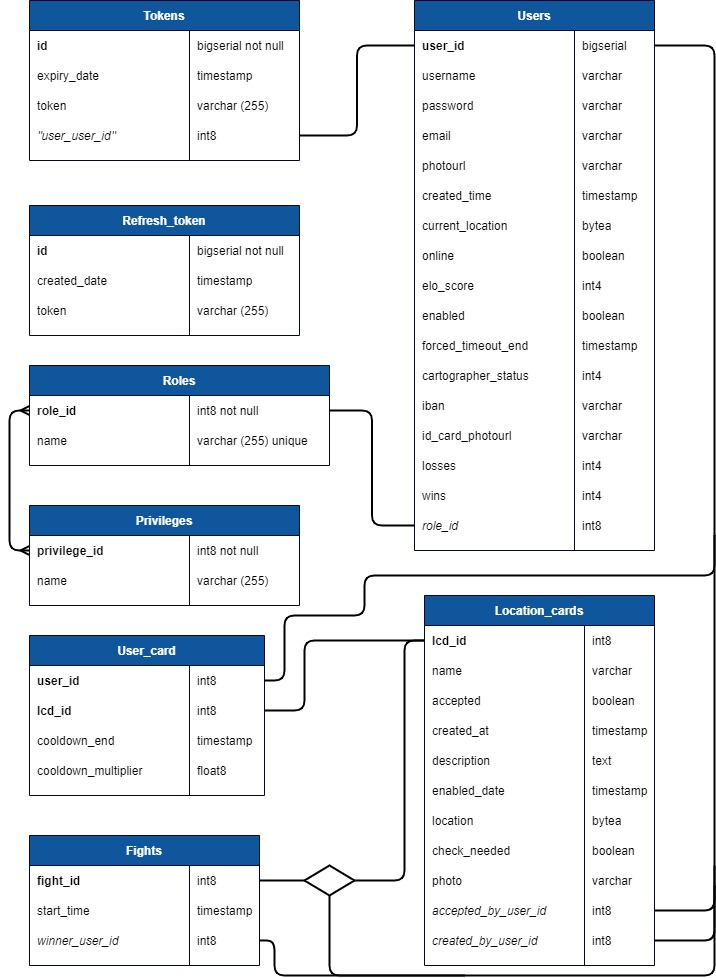
\includegraphics[scale=0.55]{slike/GeoFighterModel} 
					\caption{ER dijagram baze podataka}
					\label{fig:ERmodel}
				\end{figure}				
				
				
			
			\eject
			
			
		\section{Dijagram razreda}
		
			
			\textnormal{Na slikama 4.5, 4.6, 4.7 i 4.8 su prikazani razredi i sučelja koji pripadaju \textit{back-end} servisu izrađenom koristeći programski okvir SpringBoot i programski jezik Java. Svi razredi imaju implementirane get i set metode za vlastite atribute iako se to eksplicitno ne navodi na dijagramima.} \\
			
			\begin{figure}[H]
				\centering
				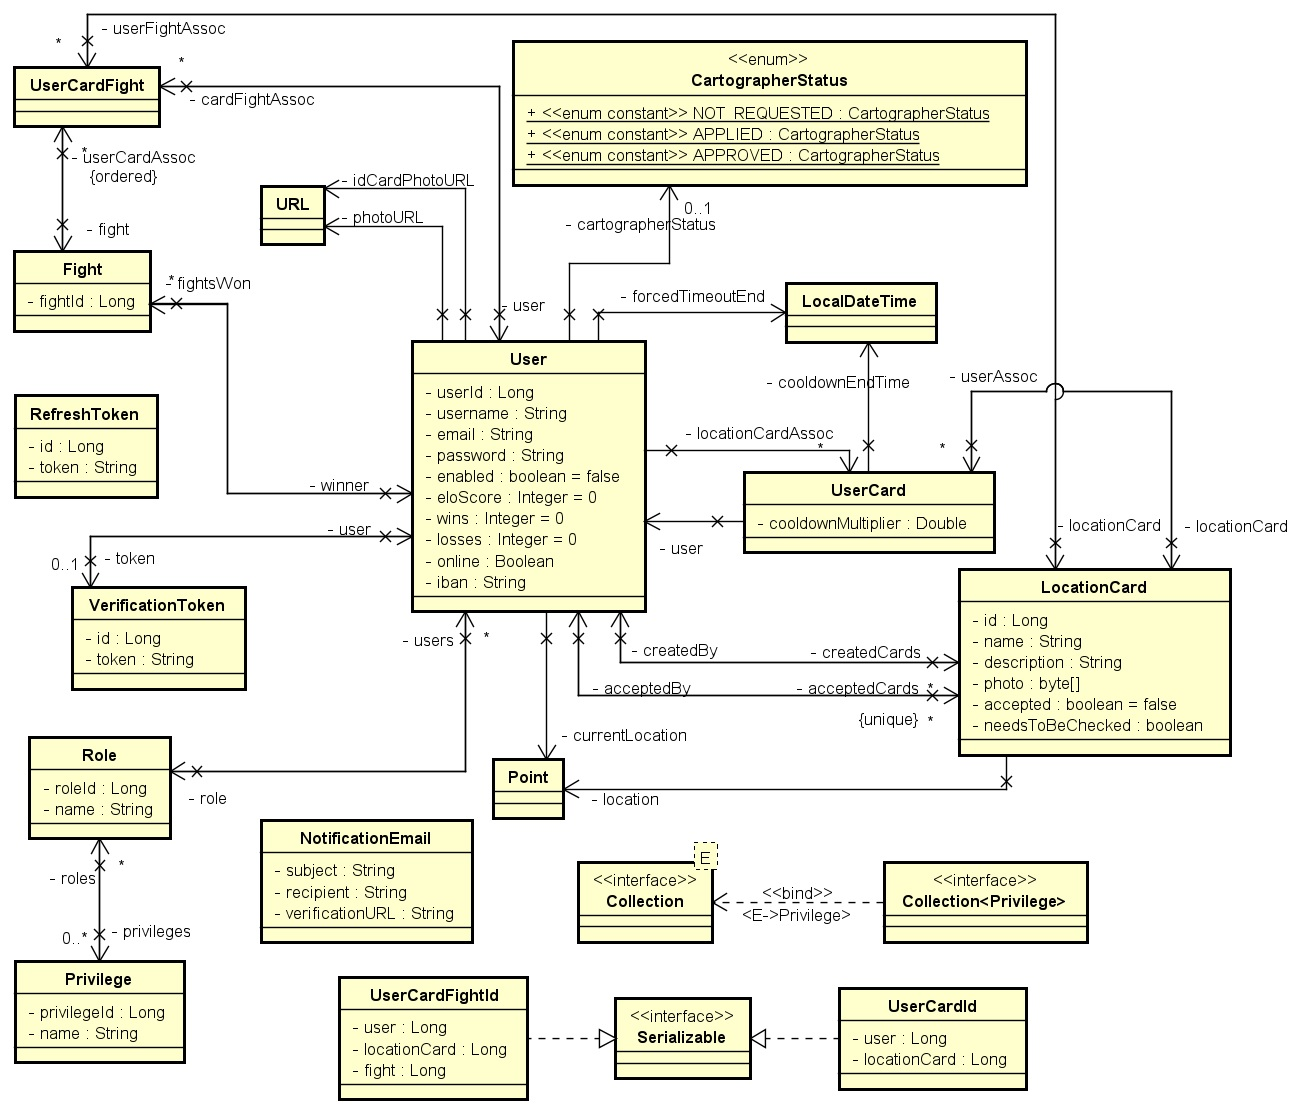
\includegraphics[scale=0.75]{slike/modelCD} \\
				\caption{ Model razredi}
				\label{fig:modelCD}
			\end{figure}
		
			\textnormal{Model razredi prikazani na slici 4.5 preslikavaju strukturu baze podataka u aplikaciji. Implementirane metode direktno komuniciraju s bazom podataka te vraćaju tražene podatke. Razred User predstavlja korisnika koji se može registrirati u sustav koristeći osnovne informacije. Razred LocationCard predstavlja karticu lokacije, dok razred UserCard predstavlja posjedovanje same kartice od strane nekog korisnika.} \\
			
			\begin{figure}[H]
				\centering
				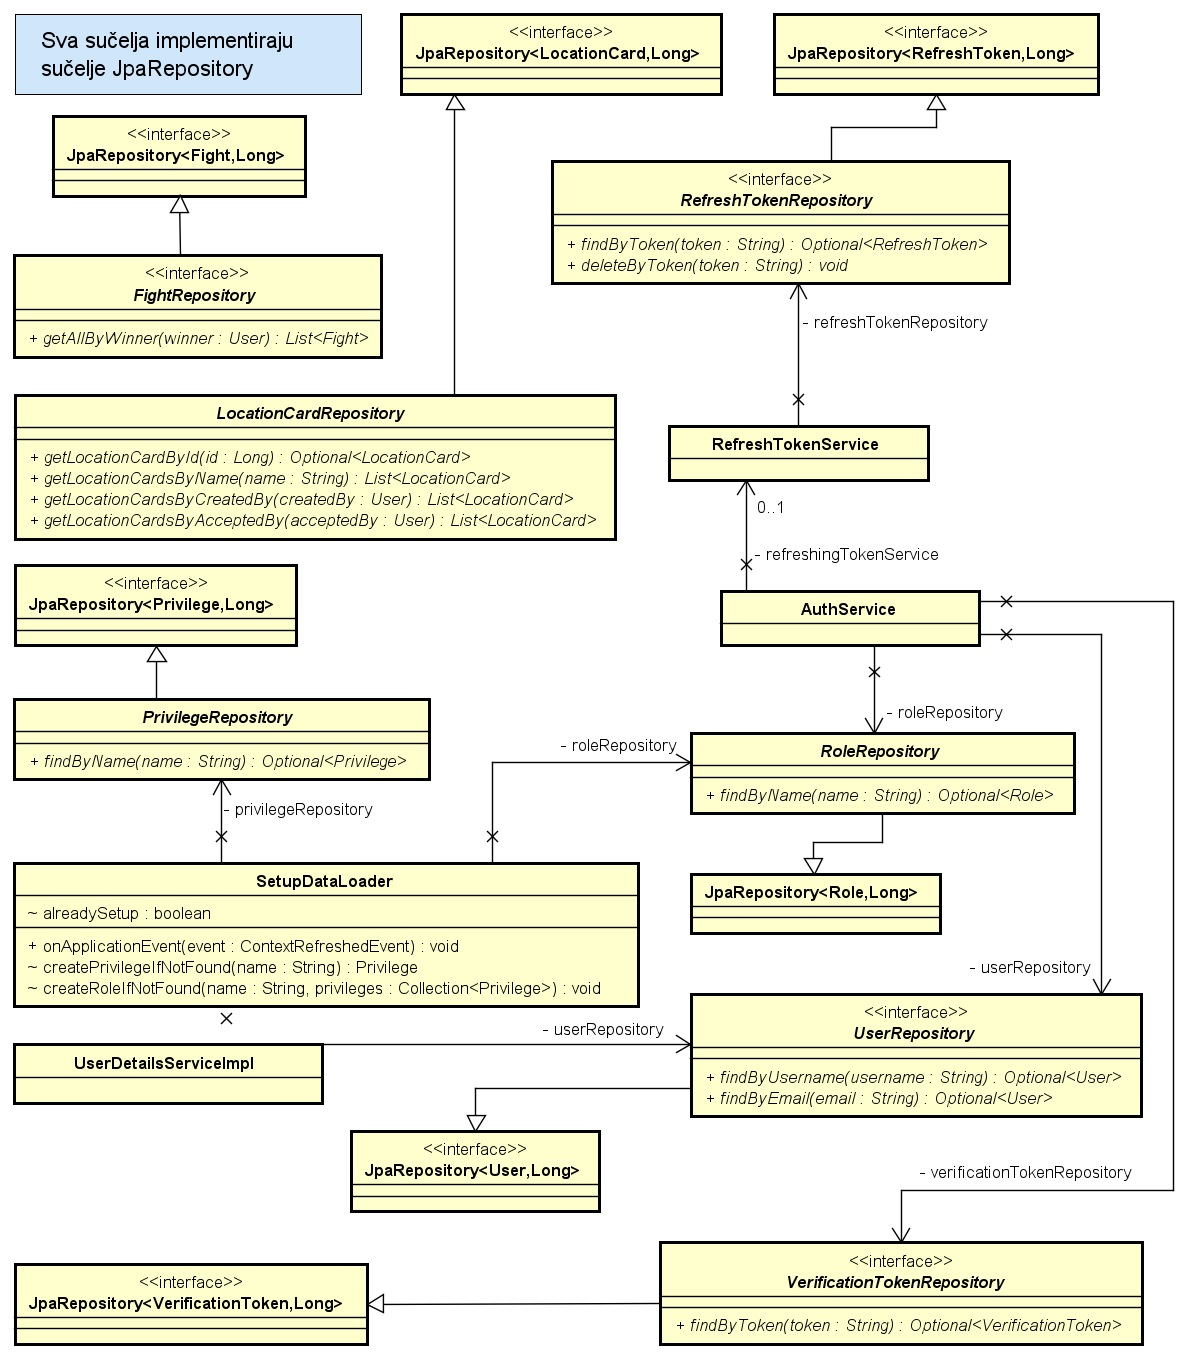
\includegraphics[scale=0.7]{slike/suceljaCD} \\
				\caption{ Dijagram sučelja sustava i razreda koji ih implementiraju}
				\label{fig:suceljaCD}
			\end{figure}
		
				\textnormal{Na slici 4.6 prikazana su sučelja i razredi koji ih implemenentiraju. Zbog bolje preglednosti dijagrama razredi su navedeni isključivo imenom, a njihov detaljan opis nalazi se na slici 4.7.} \\
						
			\begin{figure}[H]
				\centering
				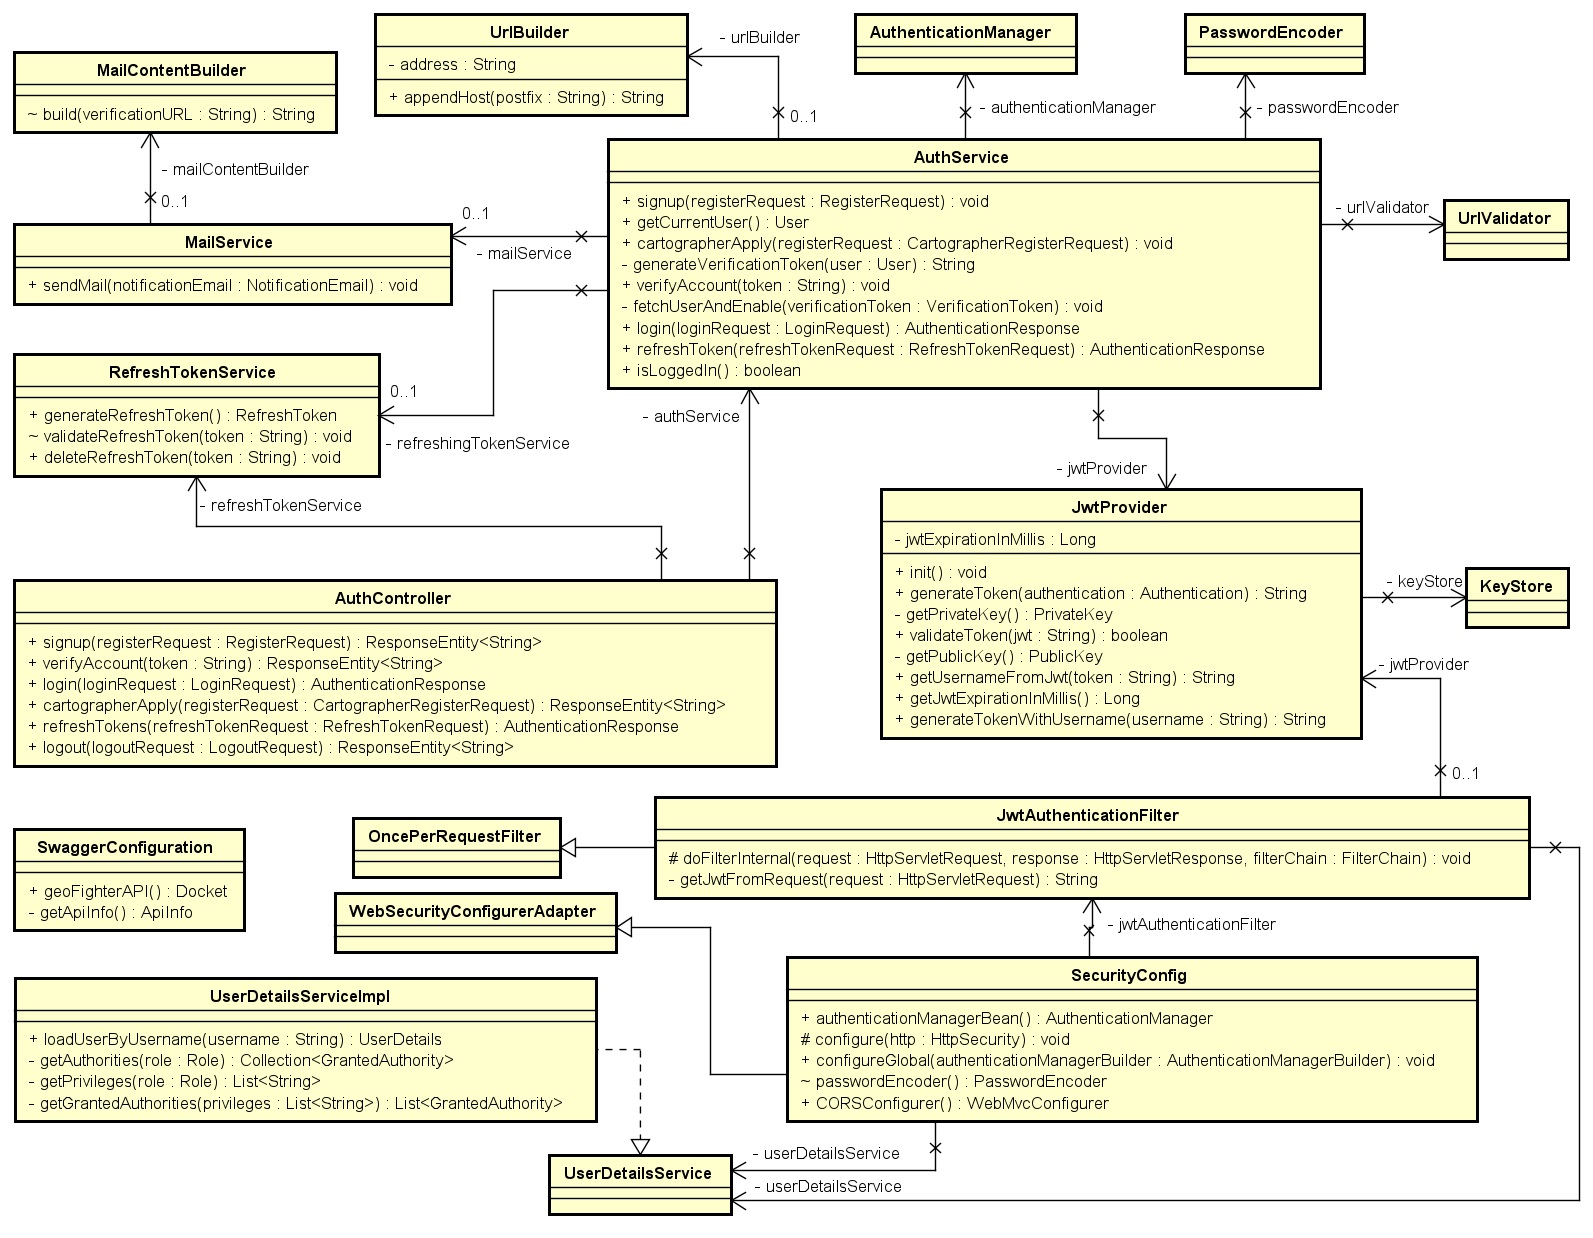
\includegraphics[scale=0.6]{slike/ostaloCD} \\
				\caption{ Dijagram razreda za upravljanje registracijom i prijavom}
				\label{fig:ostaloCD}
			\end{figure}
		
			\textnormal{Na slici 4.7 nalaze se preostali razredi sustava. Razred AuthController uz razrede AuthService, RefreshTokenService i UserDetailServiceImpl upravlja procesom registracije i prijave.} \\
			
			\textnormal{Na slici 4.8 prikazani su DTO (Data transfer object) razredi te razredi stvorenih iznimki. DTO klase služe sa prijenos podataka prilikom registracije, prijave i odjave iz sustava. }
			
			\begin{figure}[H]
				\centering
				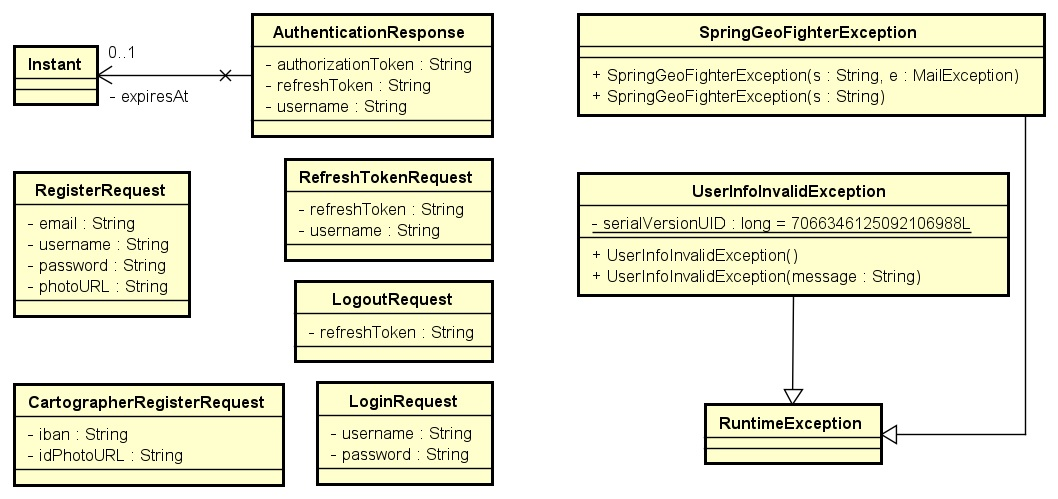
\includegraphics[scale=0.75]{slike/dtoCD} \\
				\caption{ DTO razredi i razredi iznimki}
				\label{fig:dtoCD}
			\end{figure}
			
			\textnormal{Na slijedećim slikama nalaze se razredi koje ćemo tek implementirati. Na slici 4.9 nalaze se budući DTO razredi, dok se na slici 4.10 nalaze budući Service i Controller razredi.}
			
			\begin{figure}[H]
				\centering
				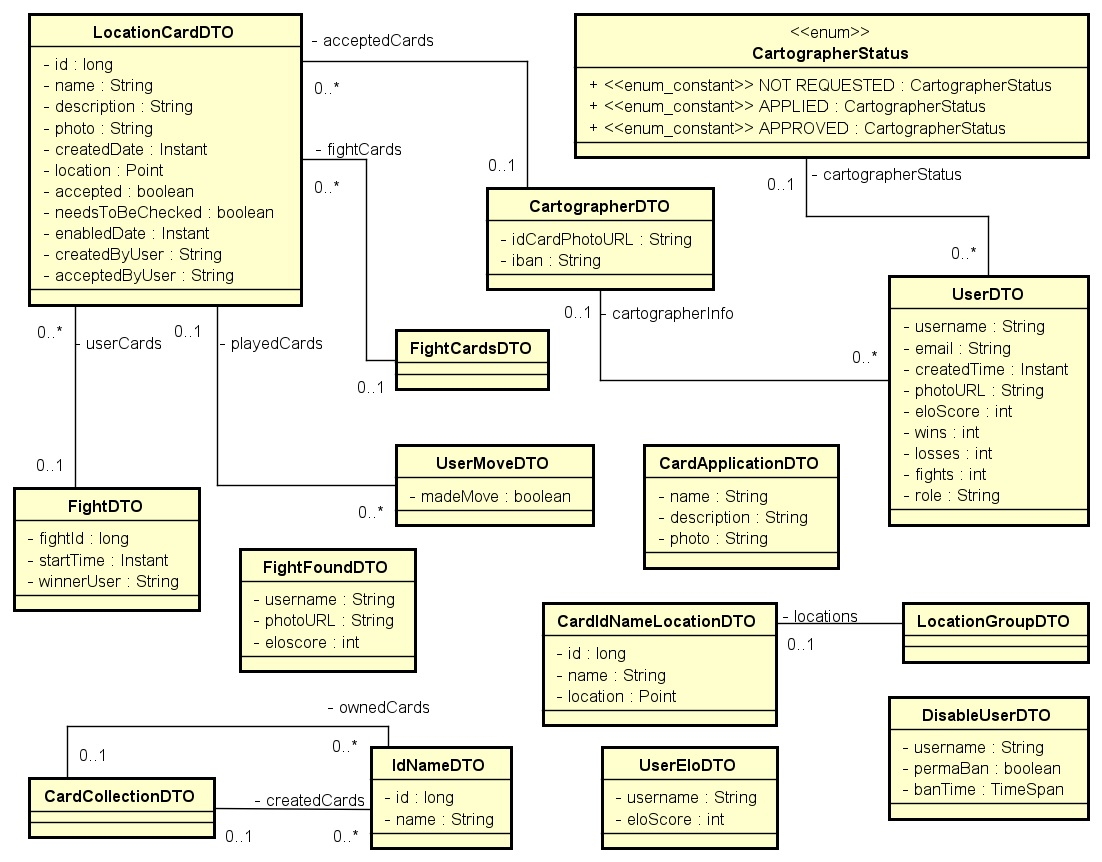
\includegraphics[scale=0.75]{slike/buduciDTO} \\
				\caption{ Budući DTO razredi}
				\label{fig:dtoBuduci}
			\end{figure}
		
			\begin{figure}[H]
				\centering
				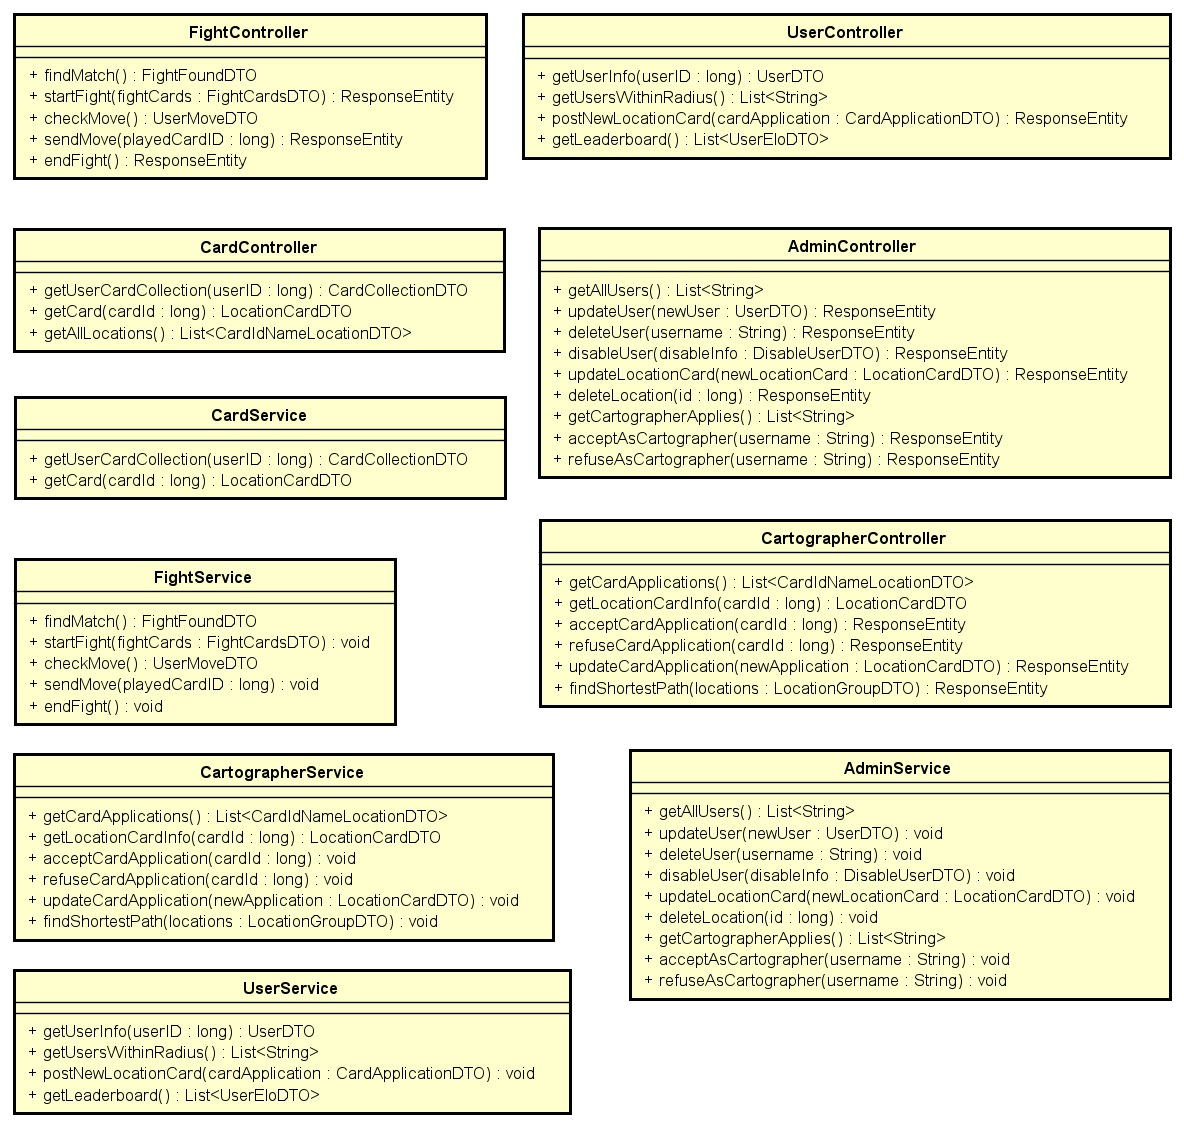
\includegraphics[scale=0.75]{slike/buduciControllerService} \\
				\caption{ Budući Controller i Service razredi}
				\label{fig:dtoCiS}
			\end{figure}
			
			\eject
		
		\section{Dijagram stanja}
			
			
			\textbf{\textit{dio 2. revizije}}\\
			
			\textit{Potrebno je priložiti dijagram stanja i opisati ga. Dovoljan je jedan dijagram stanja koji prikazuje \textbf{značajan dio funkcionalnosti} sustava. Na primjer, stanja korisničkog sučelja i tijek korištenja neke ključne funkcionalnosti jesu značajan dio sustava, a registracija i prijava nisu. }
			
			
			\eject 
		
		\section{Dijagram aktivnosti}
			
			\textbf{\textit{dio 2. revizije}}\\
			
			 \textit{Potrebno je priložiti dijagram aktivnosti s pripadajućim opisom. Dijagram aktivnosti treba prikazivati značajan dio sustava.}
			
			\eject
		\section{Dijagram komponenti}
		
			\textbf{\textit{dio 2. revizije}}\\
		
			 \textit{Potrebno je priložiti dijagram komponenti s pripadajućim opisom. Dijagram komponenti treba prikazivati strukturu cijele aplikacije.}